\chapter{System Design}
\label{chap:system-design}
\textit{This chapter designs the system that meets the requirements of Chapter~\ref{chap:requirements}: the behavioral models that refine the use cases; the architecture, the alternatives considered and the way it realizes the non-functional requirements; the database, the API and the user interface; and, finally, the traceability from every functional requirement to the design.}

\section{Behavioral Design}
\label{sec:sd-behavior}

\subsection{Run Lifecycle}
\label{sec:sd-run-lifecycle}

Work starts from the chat box: creating a thread starts nothing, the first message does. The first run of a project begins at the planner, and every later run, in any thread of the project, begins at the intent router (Figure~\ref{fig:sd-run-entry}).

\begin{figure}[H]
    \centering
    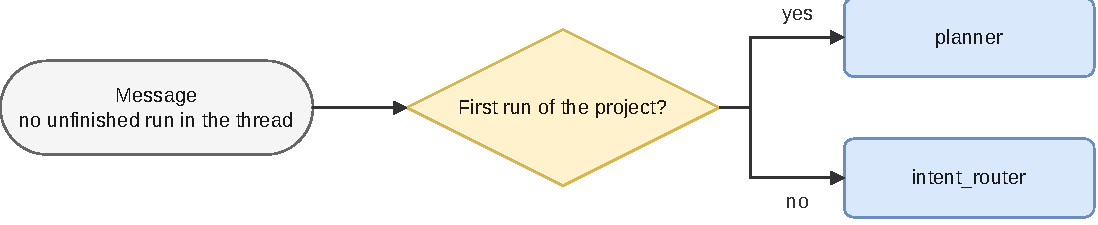
\includegraphics[width=0.75\linewidth]{system-design/runtime-run-entry.pdf}
    \caption{Where a run begins in the workflow.}
    \label{fig:sd-run-entry}
\end{figure}

A run is a resource with a lifecycle (Figure~\ref{fig:sd-run-lifecycle}). It is \emph{unfinished} while it is \texttt{queued}, \texttt{running} or \texttt{interrupted}, and \emph{finished} once it is \texttt{succeeded}, \texttt{failed} or \texttt{cancelled}; a finished run never changes status again. An interrupted run waits for the user at a checkpoint with no time limit. A thread has at most one unfinished run.

\begin{figure}[H]
    \centering
    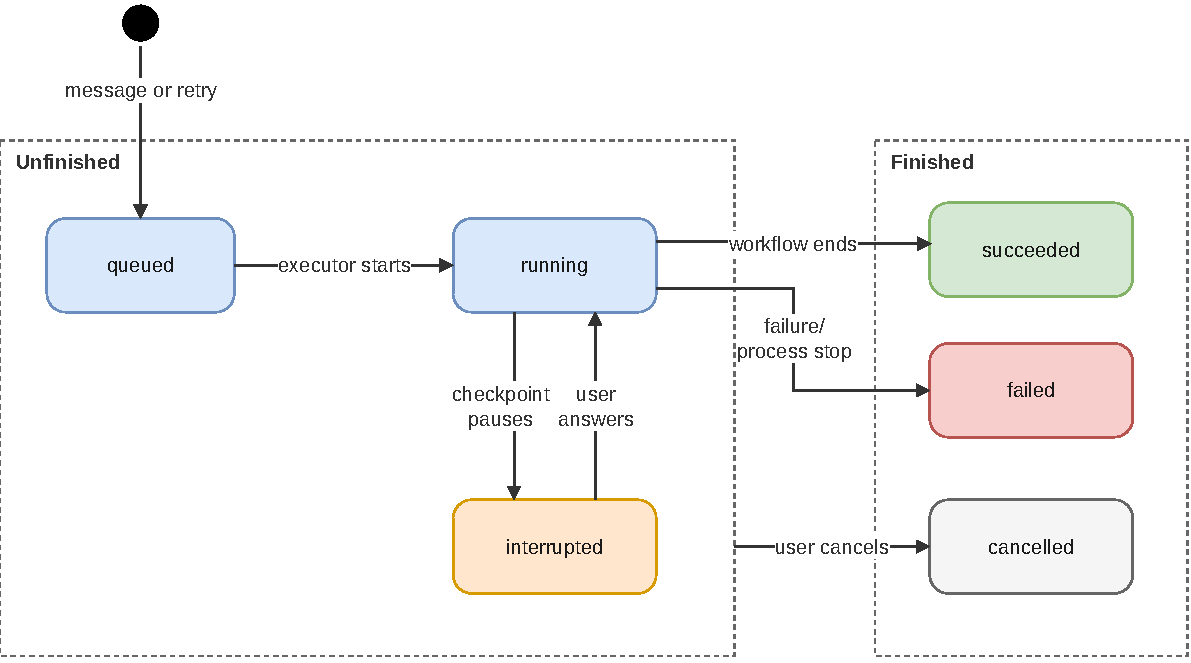
\includegraphics[width=0.7\linewidth]{system-design/runtime-run-lifecycle.pdf}
    \caption{State diagram of a run.}
    \label{fig:sd-run-lifecycle}
\end{figure}

\subsection{Steps of a Node}
\label{sec:sd-node-steps}

Figure~\ref{fig:sd-node-steps} shows what happens at every node of a run. Before a node calls an LLM, the cost limit of the run and the budget of the user are checked, so that a run fails before it overspends rather than after. The node then calls the model, writes its items through the integrity checks, and appends its events to the event log. At a checkpoint node the run is interrupted until the user chooses an option. After each node the state is saved: this \emph{safe point} is where a failed run can be retried from, and where pending user messages are taken in by the intent router.

\begin{figure}[H]
    \centering
    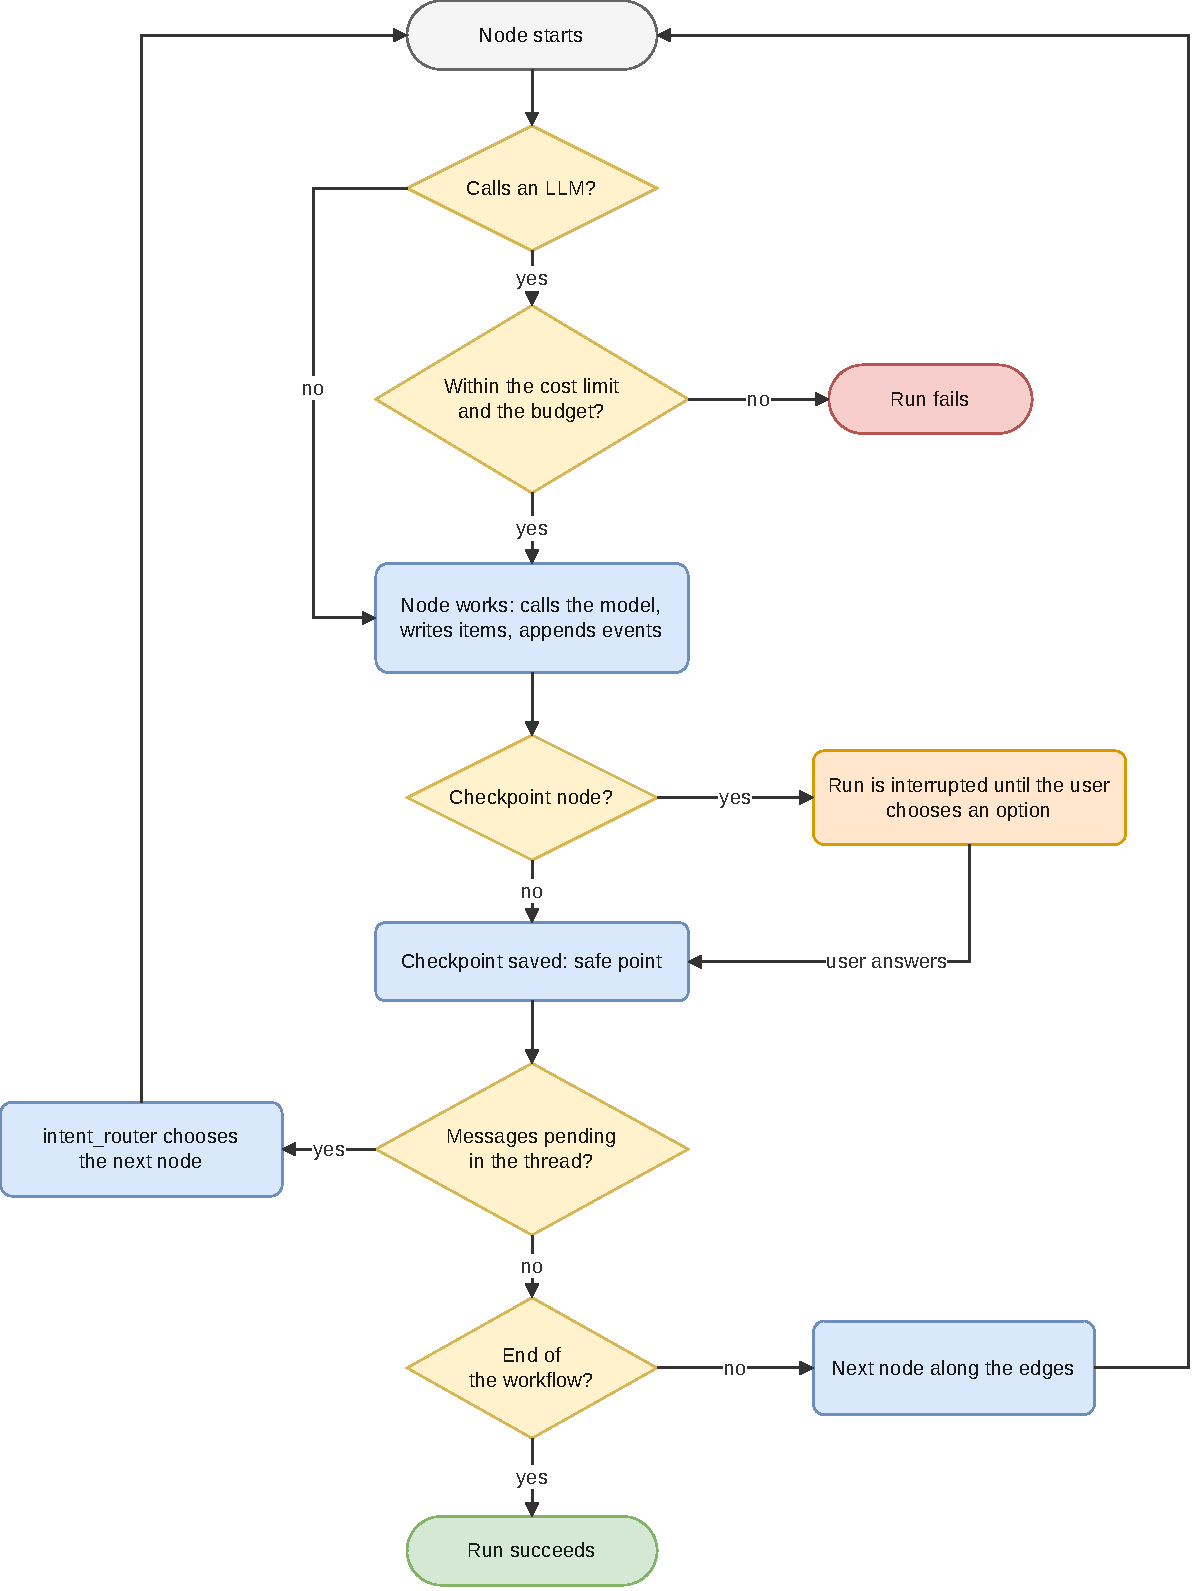
\includegraphics[height=0.62\textheight]{system-design/runtime-node-steps.pdf}
    \caption{Activity diagram of one node of a run.}
    \label{fig:sd-node-steps}
\end{figure}

\subsection{Messages During a Run}
\label{sec:sd-messages}

A message the user sends while a run is unfinished is stored as \emph{pending}. It becomes \emph{delivered} when the intent router takes it in at the next safe point, and \emph{undelivered} if the run fails or is cancelled first, in which case the user can send it again (Figure~\ref{fig:sd-message-delivery}). A message sent when no run is unfinished starts a new run.

\begin{figure}[H]
    \centering
    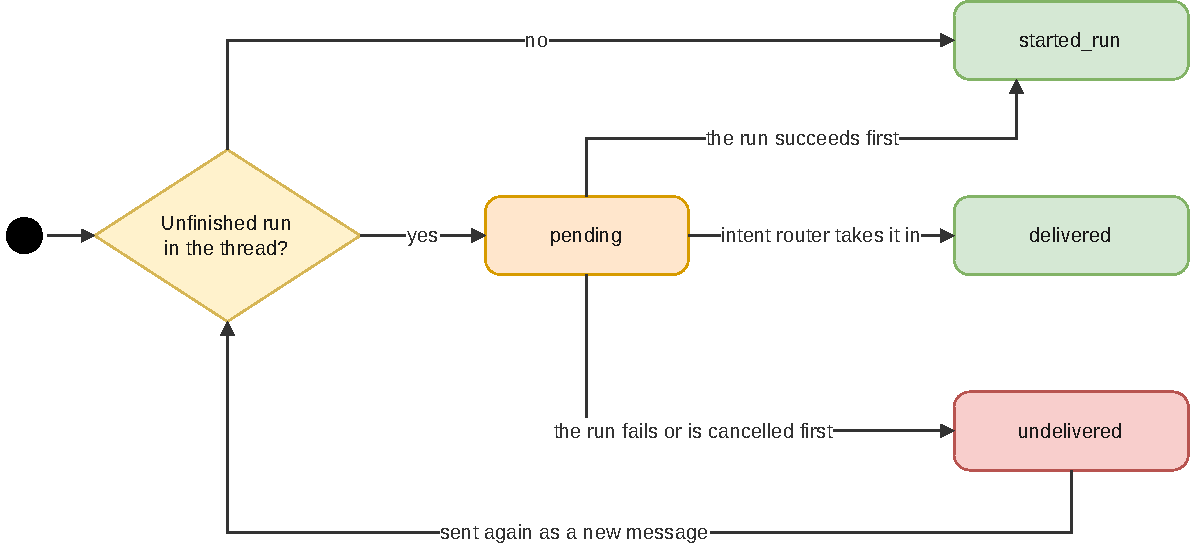
\includegraphics[width=0.75\linewidth]{system-design/runtime-message-delivery.pdf}
    \caption{State diagram of a user message.}
    \label{fig:sd-message-delivery}
\end{figure}

\subsection{Sequence of a Run}
\label{sec:sd-sequence}

Figure~\ref{fig:sd-sequence} shows the interactions of use case UC-01 and UC-02. The essential property is that the workflow never writes into an HTTP response: it appends events to the event log in the database, and the stream endpoint reads the log. The request that starts a run therefore returns at once, a closed browser does not stop the run, and a client that reconnects receives the events it missed by sending the identifier of the last event it saw.

\begin{figure}[H]
    \centering
    \resizebox{\linewidth}{!}{%
    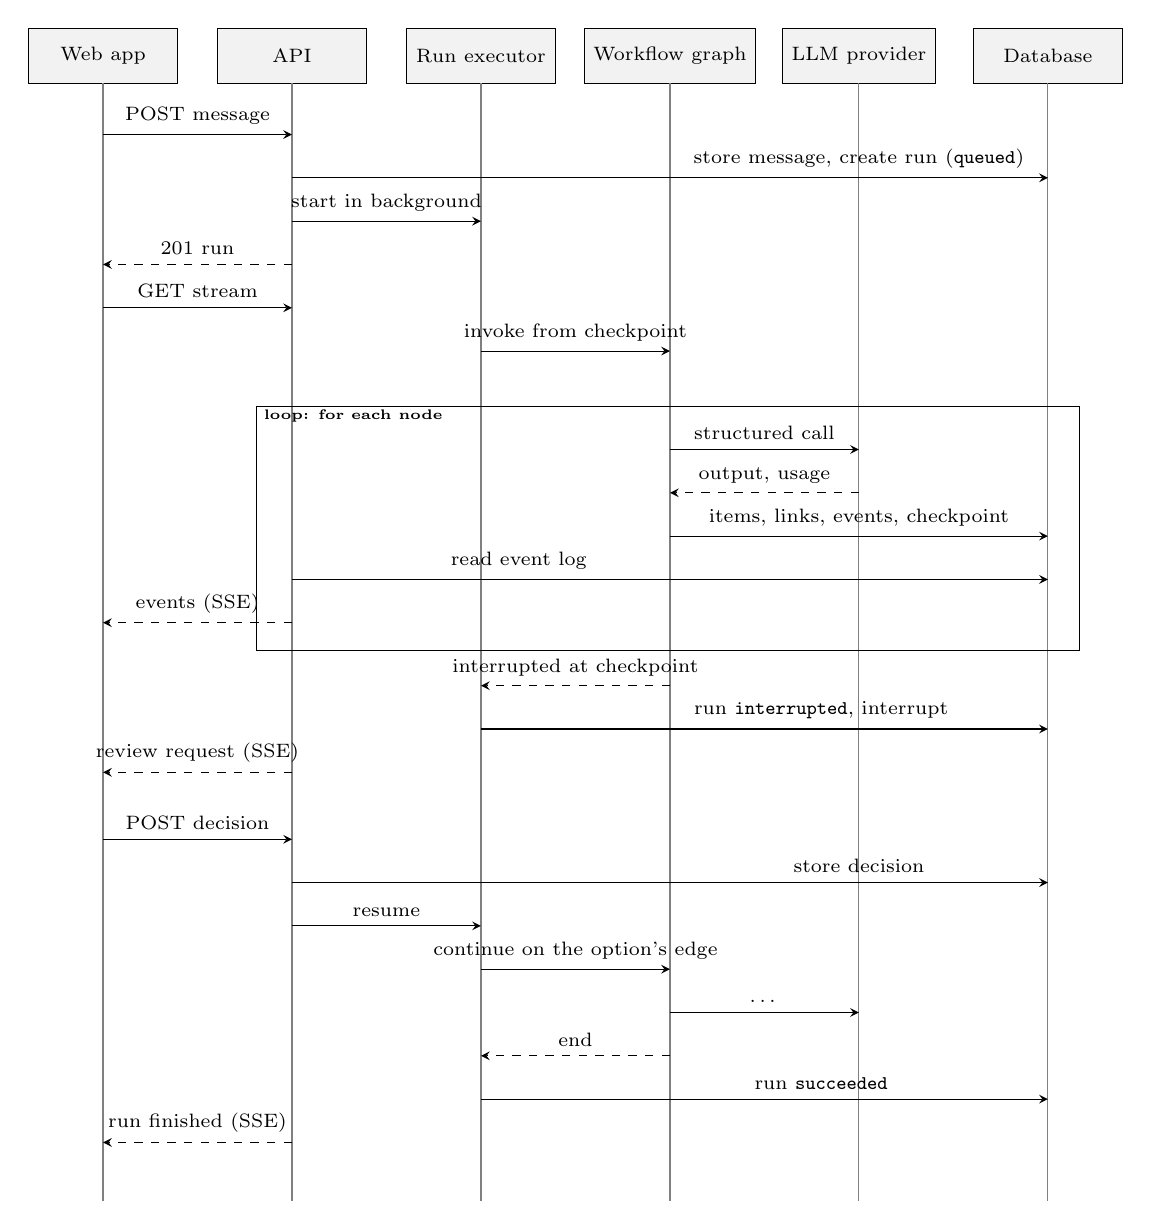
\begin{tikzpicture}[
        font=\scriptsize,
        life/.style={draw, fill=gray!10, minimum width=1.9cm, minimum height=0.7cm, align=center},
        msg/.style={->, >=stealth},
        ret/.style={->, >=stealth, dashed}
    ]
        \foreach \name/\label/\x in {web/Web app/0, api/API/2.4, exe/Run executor/4.8, graph/Workflow graph/7.2, llm/LLM provider/9.6, db/Database/12.0} {
            \node[life] (\name) at (\x, 0) {\label};
            \draw[gray] (\x, -0.35) -- (\x, -14.55);
        }
        \draw[msg] (0,-1.00) -- node[above] {POST message} (2.4,-1.00);
        \draw[msg] (2.4,-1.55) -- node[above, pos=0.75] {store message, create run (\texttt{queued})} (12.0,-1.55);
        \draw[msg] (2.4,-2.10) -- node[above] {start in background} (4.8,-2.10);
        \draw[ret] (2.4,-2.65) -- node[above] {201 run} (0,-2.65);
        \draw[msg] (0,-3.20) -- node[above] {GET stream} (2.4,-3.20);
        \draw[msg] (4.8,-3.75) -- node[above] {invoke from checkpoint} (7.2,-3.75);
        \node[font=\tiny\bfseries, anchor=north west, inner sep=1pt] at (2.0,-4.45) {loop: for each node};
        \draw[msg] (7.2,-5.00) -- node[above] {structured call} (9.6,-5.00);
        \draw[ret] (9.6,-5.55) -- node[above] {output, usage} (7.2,-5.55);
        \draw[msg] (7.2,-6.10) -- node[above] {items, links, events, checkpoint} (12.0,-6.10);
        \draw[msg] (2.4,-6.65) -- node[above, pos=0.3] {read event log} (12.0,-6.65);
        \draw[ret] (2.4,-7.20) -- node[above] {events (SSE)} (0,-7.20);
        \draw (1.95,-4.45) rectangle (12.4,-7.55);
        \draw[ret] (7.2,-8.00) -- node[above] {interrupted at checkpoint} (4.8,-8.00);
        \draw[msg] (4.8,-8.55) -- node[above, pos=0.6] {run \texttt{interrupted}, interrupt} (12.0,-8.55);
        \draw[ret] (2.4,-9.10) -- node[above] {review request (SSE)} (0,-9.10);
        \draw[msg] (0,-9.95) -- node[above] {POST decision} (2.4,-9.95);
        \draw[msg] (2.4,-10.50) -- node[above, pos=0.75] {store decision} (12.0,-10.50);
        \draw[msg] (2.4,-11.05) -- node[above] {resume} (4.8,-11.05);
        \draw[msg] (4.8,-11.60) -- node[above] {continue on the option's edge} (7.2,-11.60);
        \draw[msg] (7.2,-12.15) -- node[above] {\ldots} (9.6,-12.15);
        \draw[ret] (7.2,-12.70) -- node[above] {end} (4.8,-12.70);
        \draw[msg] (4.8,-13.25) -- node[above, pos=0.6] {run \texttt{succeeded}} (12.0,-13.25);
        \draw[ret] (2.4,-13.80) -- node[above] {run finished (SSE)} (0,-13.80);
    \end{tikzpicture}}
    \caption{Sequence diagram of starting a run and answering a checkpoint (UC-01 and UC-02).}
    \label{fig:sd-sequence}
\end{figure}

\subsection{Failures, Cancellation and Restarts}
\label{sec:sd-failures}

A step that fails, for example because a provider returns an error or an agent output fails the integrity checks, ends the run as \texttt{failed} with an error code. The user can retry it: the retry starts a new run from the last completed step, using the saved checkpoint, so the LLM calls of earlier steps are not made again. Cancellation stops the run at the next safe point. Since runs execute as tasks inside the API process, a restart of the process ends the steps in progress: on startup the API marks those runs as \texttt{failed} with the code \texttt{server\_restarted}, starts again the runs that were still \texttt{queued}, and leaves interrupted runs waiting for the user.

\section{System Architecture}
\label{sec:sd-architecture}

The structure diagrams follow the building block view of arc42, equivalent to the context, container and component levels of the C4 model; together with the behavior, deployment and database diagrams they cover the views of the 4+1 model~\cite{kruchten1995}.

\subsection{Building Blocks}
\label{sec:sd-building-blocks}

\begin{figure}[H]
    \centering
    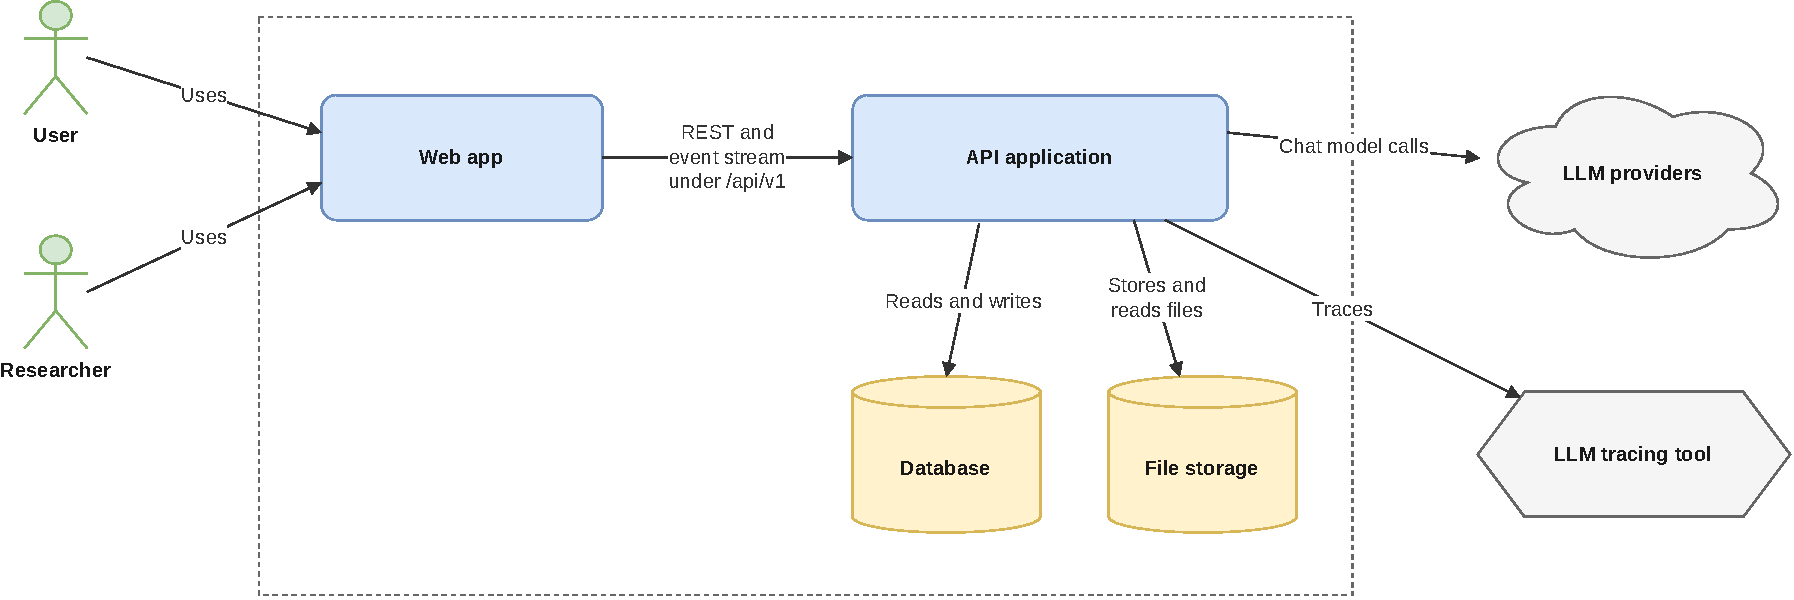
\includegraphics[width=\linewidth]{system-design/building-blocks.pdf}
    \caption{Building blocks of the system.}
    \label{fig:sd-building-blocks}
\end{figure}

\begin{itemize}
    \item \textbf{Web app}: chat, workflow graph, artifact panel and settings. It holds no business logic and draws the workflow and the artifacts from data the API provides.
    \item \textbf{API application}: REST and event stream API, authentication, execution of the agent workflow as background tasks, calls to the LLM providers.
    \item \textbf{Database}: application data, run events, workflow checkpoints and vectors.
    \item \textbf{File storage}: exported documents and uploaded files.
\end{itemize}
The workflow writes its events to an event log in the database and the stream endpoint reads the log; the workflow never writes into an HTTP response, so a closed browser does not stop a run and a reconnecting client gets the events it missed.

\subsection{Backend Modules}
\label{sec:sd-backend-modules}
The API application is one deployable unit, a modular monolith. Figure~\ref{fig:sd-backend-modules} shows its modules and the allowed import directions.

\begin{figure}[H]
    \centering
    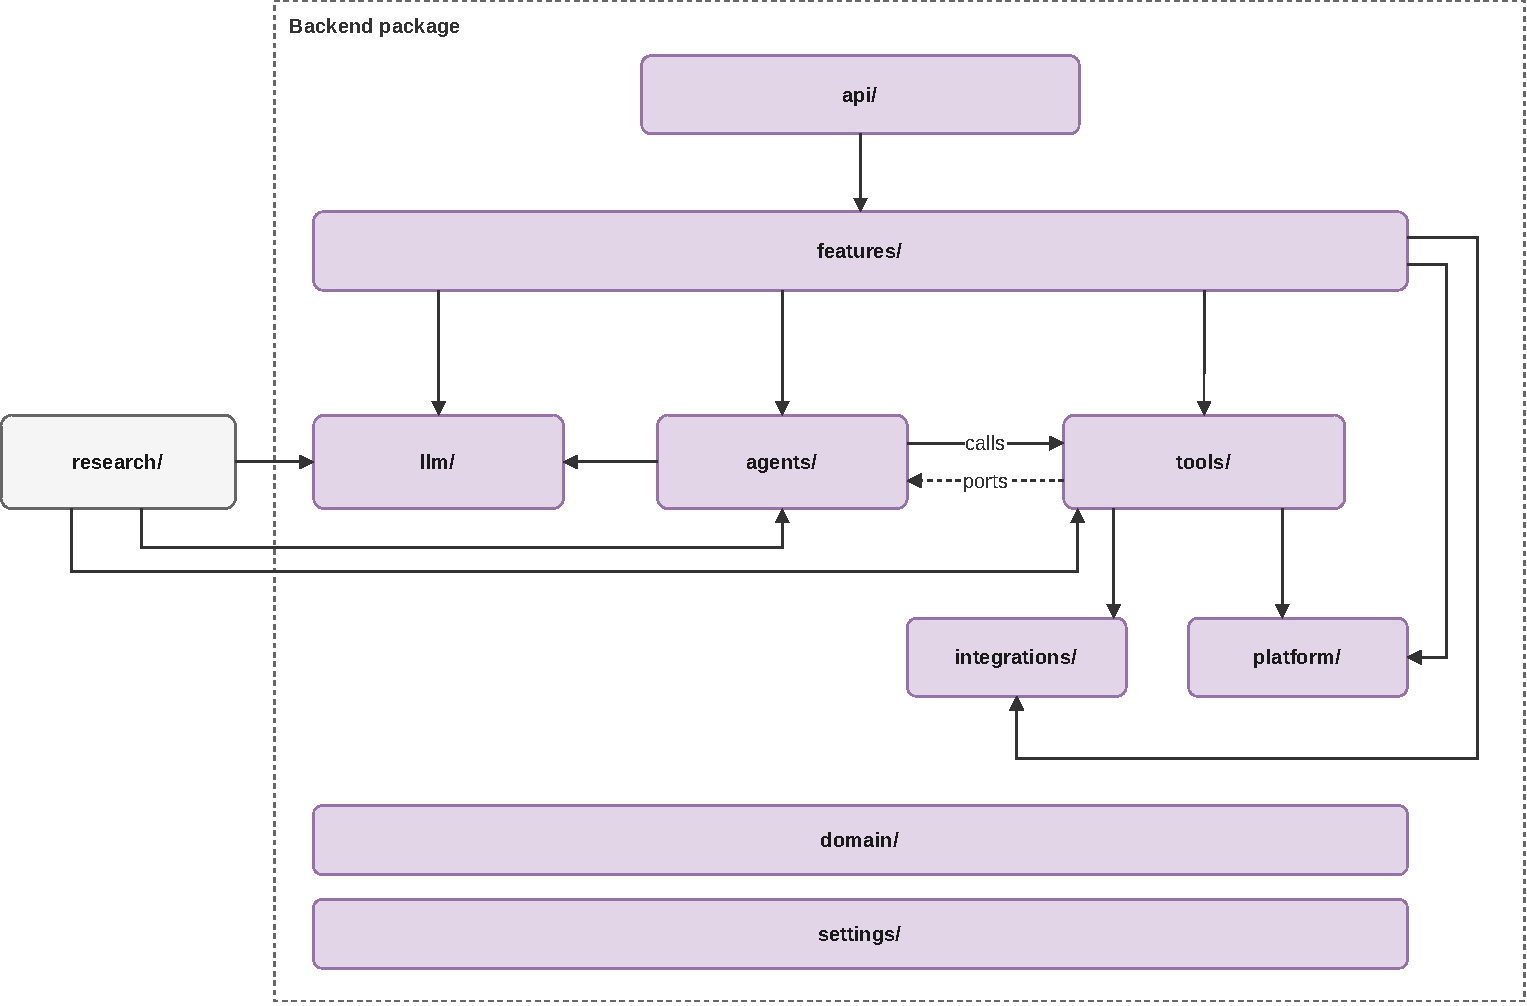
\includegraphics[width=0.85\linewidth]{system-design/backend-modules.pdf}
    \caption{Backend modules and allowed import directions.}
    \label{fig:sd-backend-modules}
\end{figure}

\begin{table}[H]
    \centering
    \caption{Responsibilities of the backend modules.}
    \label{tab:sd-backend-modules}
    \begin{tabularx}{\linewidth}{|l|X|}
        \hline
        \textbf{Module} & \textbf{Responsibility} \\
        \hline
        \texttt{api/} & Mounts the feature routers under \texttt{/api/v1}; maps domain errors to HTTP responses \\
        \texttt{features/} & One package per business feature (auth, projects, threads, runs, artifacts, model settings), each with a router, schemas, a service, a repository and models \\
        \texttt{agents/} & The workflow graph: state, nodes, prompts, ports, and the versioned workflow definition \\
        \texttt{llm/} & The only place that creates chat models; resolves an agent role to a provider and a model; checks cost limits and records usage around every call \\
        \texttt{tools/} & Tools that agents can call, such as research search \\
        \texttt{platform/} & Database session, object storage client, background run executor \\
        \texttt{domain/} & Business rules without infrastructure: content schemas, integrity rules, domain errors \\
        \texttt{settings/} & Application settings and logging \\
        \texttt{research/} & Evaluation harness, outside the backend, importing the same agents \\
        \hline
    \end{tabularx}
\end{table}

\subsection{Frontend Architecture}
\label{sec:sd-frontend}

\begin{figure}[H]
    \centering
    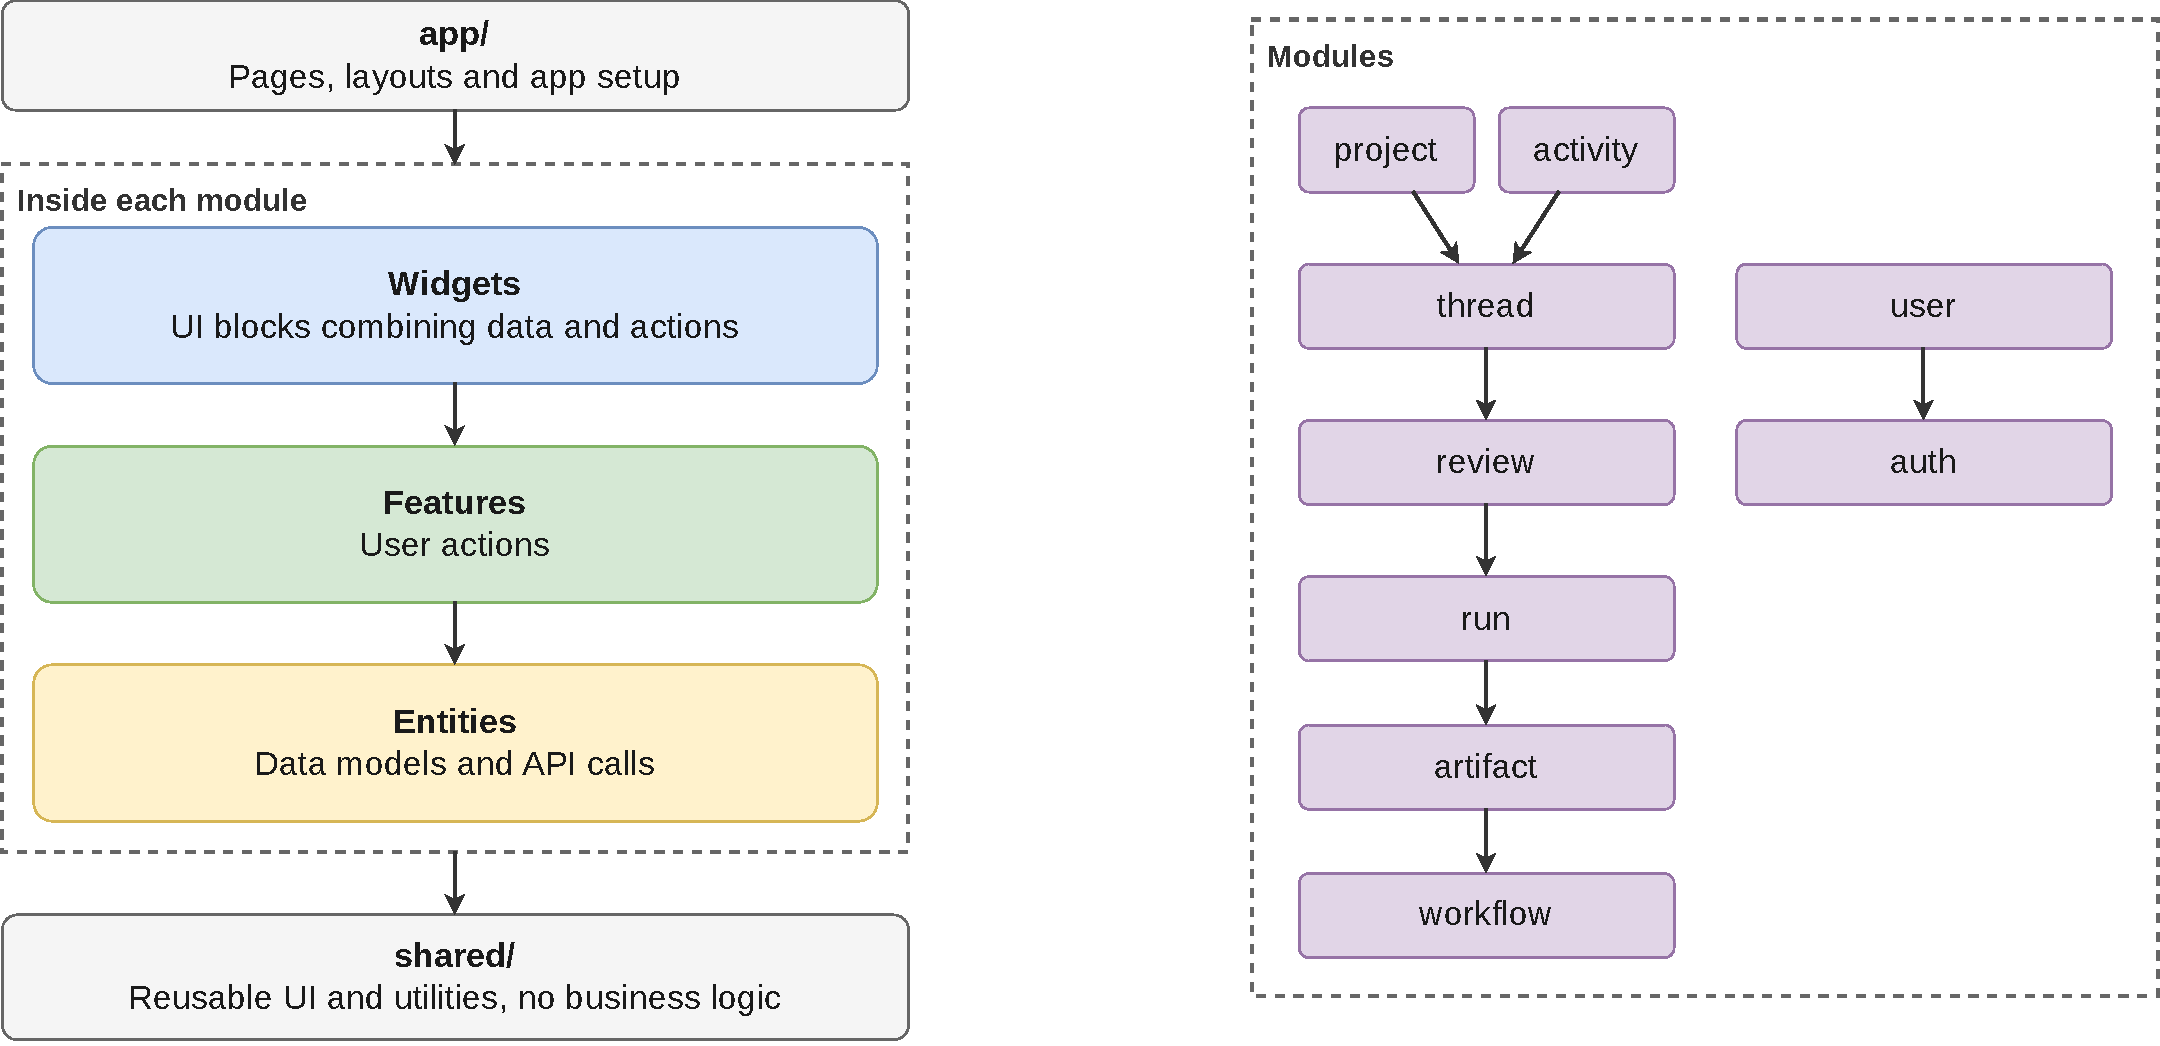
\includegraphics[width=\linewidth]{system-design/frontend-architecture.pdf}
    \caption{Frontend architecture.}
    \label{fig:sd-frontend}
\end{figure}
\todo{Describe the layers of the web app: routes, features, typed API client generated from the OpenAPI schema, server state and client state.}

\subsection{Deployment}
\label{sec:sd-deployment}

\begin{figure}[H]
    \centering
    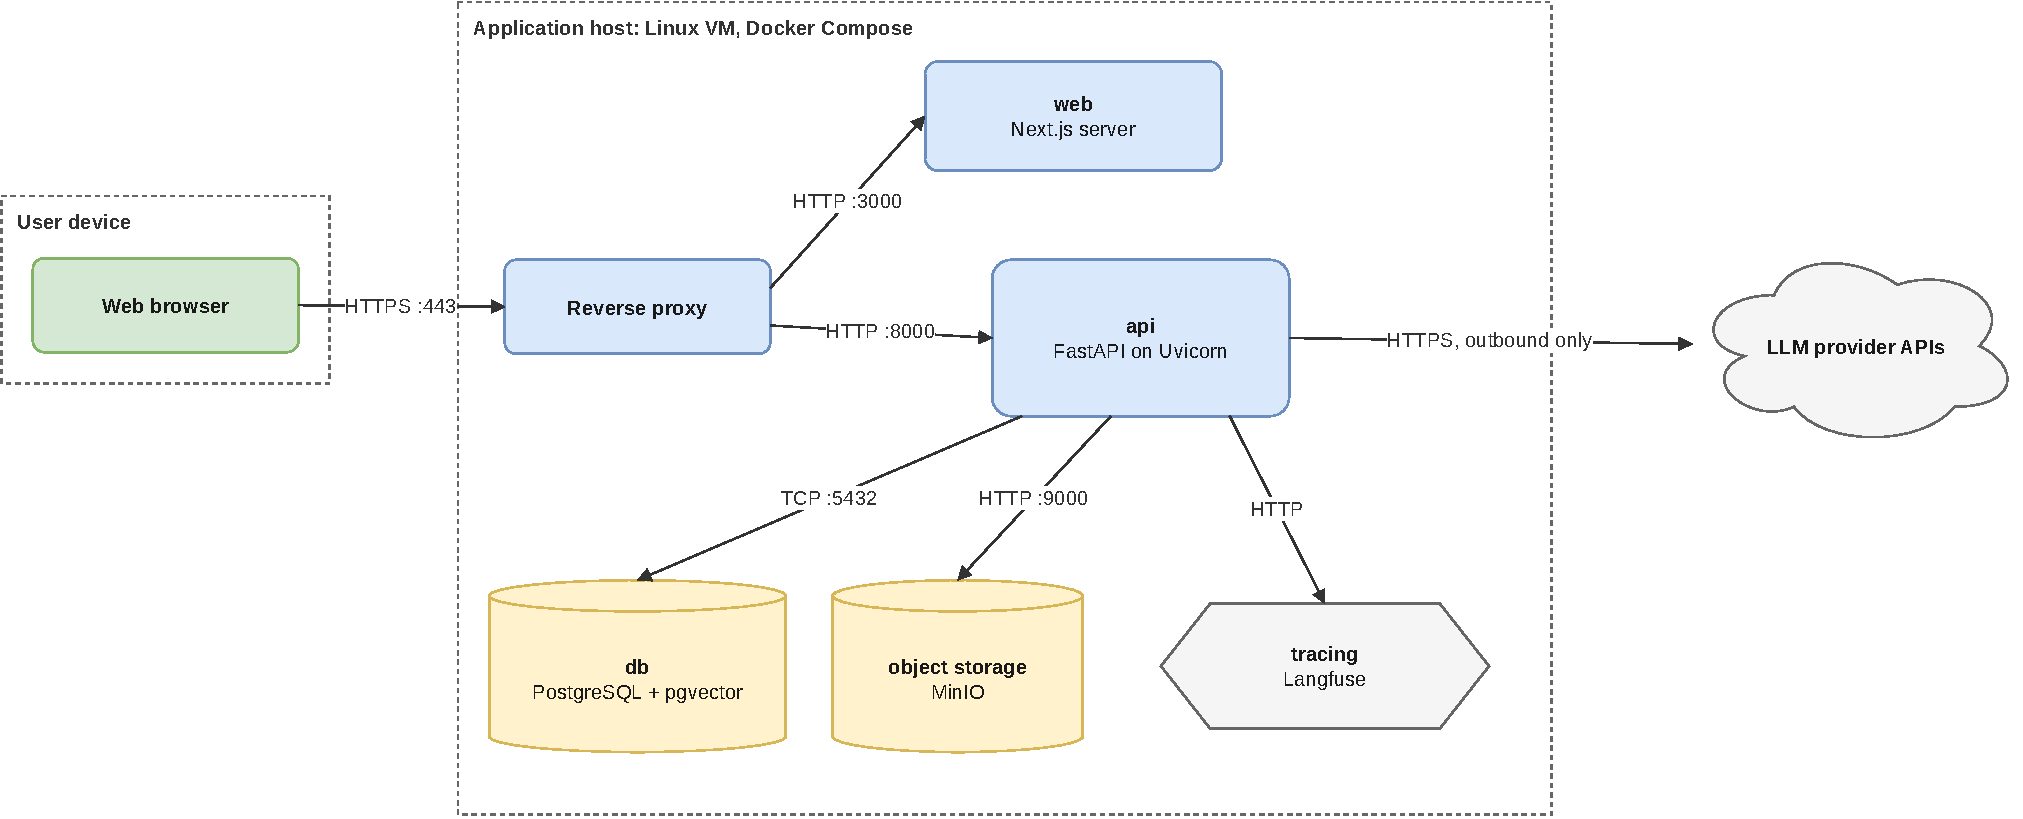
\includegraphics[width=\linewidth]{system-design/deployment-production.pdf}
    \caption{Deployment diagram (production).}
    \label{fig:sd-deployment}
\end{figure}
\todo{Describe the nodes (reverse proxy, web, api, db, object storage, tracing) and the constraints: same origin, one API process, long-lived responses.}

\section{Database Design}
\label{sec:sd-database}

The schema has 24 tables in five groups (Table~\ref{tab:sd-tables}). Figure~\ref{fig:sd-domain-model} shows the main persistent entities and their associations as a UML class diagram; tables that only support these entities (sessions, settings, revisions and exports) are left out.

\begin{figure}[H]
    \centering
    \resizebox{\linewidth}{!}{% UML class diagram of the main persistent entities (Section 5.7).
\begin{tikzpicture}[uml]
    \begin{class}[text width=2.9cm]{User}{0,0}
        \attribute{id : UUID}
        \attribute{email : String}
        \attribute{display\_name : String}
    \end{class}
    \begin{class}[text width=3.1cm]{Project}{5.2,0}
        \attribute{id : UUID}
        \attribute{name : String}
        \attribute{initial\_message\_id : UUID [0..1]}
    \end{class}
    \begin{class}[text width=2.9cm]{SourceDocument}{10.4,0}
        \attribute{id : UUID}
        \attribute{title : String}
        \attribute{text : String}
    \end{class}
    \begin{class}[text width=2.9cm]{Thread}{0,-3.4}
        \attribute{id : UUID}
        \attribute{title : String}
        \attribute{current\_stage : String}
    \end{class}
    \begin{class}[text width=2.9cm]{Message}{0,-7.6}
        \attribute{id : UUID}
        \attribute{role : MessageRole}
        \attribute{content : String}
        \attribute{delivery : DeliveryStatus}
    \end{class}
    \begin{class}[text width=3.1cm]{Run}{5.2,-3.4}
        \attribute{id : UUID}
        \attribute{status : RunStatus}
        \attribute{workflow\_name : String}
        \attribute{workflow\_version : Integer}
        \attribute{run\_config : JSON}
    \end{class}
    \begin{class}[text width=3.1cm]{RunStep}{3.9,-7.6}
        \attribute{sequence : Integer}
        \attribute{node : String}
        \attribute{agent\_role : String [0..1]}
        \attribute{usage : Usage}
    \end{class}
    \begin{class}[text width=2.9cm]{RunEvent}{7.3,-7.6}
        \attribute{sequence : Integer}
        \attribute{type : String}
        \attribute{payload : JSON}
    \end{class}
    \begin{class}[text width=2.9cm]{Interrupt}{10.7,-7.6}
        \attribute{node : String}
        \attribute{options : JSON}
        \attribute{status : InterruptStatus}
    \end{class}
    \begin{class}[text width=2.9cm]{HumanDecision}{10.7,-10.8}
        \attribute{option : String}
        \attribute{feedback : String [0..1]}
        \attribute{answers : JSON}
    \end{class}
    \begin{class}[text width=3.0cm]{Artifact}{10.4,-3.4}
        \attribute{kind : String}
        \attribute{version : Integer}
        \attribute{review\_status : ReviewStatus}
        \attribute{content : JSON}
    \end{class}
    \begin{class}[text width=3.0cm]{ArtifactItem}{14.6,-3.4}
        \attribute{kind : String}
        \attribute{key : String}
        \attribute{version : Integer}
        \attribute{content : JSON}
    \end{class}
    \begin{class}[text width=3.0cm]{TraceLink}{14.6,-7.6}
        \attribute{link\_type : String}
        \attribute{source\_quote : String [0..1]}
        \attribute{target\_quote : String [0..1]}
    \end{class}

    \association{User}{members}{*}{Project}{projects}{*}
    \composition{Project}{}{*}{SourceDocument}
    \composition{Project}{}{*}{Thread}
    \composition{Thread}{}{*}{Message}
    \composition{Thread}{}{*}{Run}
    \composition{Run}{}{*}{RunStep}
    \composition{Run}{}{*}{Interrupt}
    \association{Interrupt}{}{1}{HumanDecision}{}{0..1}
    \composition{Project}{}{*}{Artifact}
    \composition{Artifact}{}{*}{ArtifactItem}
    \composition{Run}{}{*}{RunEvent}
    \draw[thick] (ArtifactItem.north) -- ++(0,0.5) -| node[pos=0.25, above, font=\tiny] {parent 0..1} ($(ArtifactItem.north)+(-0.9,0)$);
    \draw[thick, ->] ($(TraceLink.north)+(-0.5,0)$) -- node[left, font=\tiny] {source 1} ($(ArtifactItem.south)+(-0.5,0)$);
    \draw[thick, ->] ($(TraceLink.north)+(0.5,0)$) -- node[right, font=\tiny] {target 1} ($(ArtifactItem.south)+(0.5,0)$);
    \node[font=\tiny] at ($(TraceLink.north)+(-0.75,0.25)$) {*};
    \node[font=\tiny] at ($(TraceLink.north)+(0.75,0.25)$) {*};
\end{tikzpicture}
}
    \caption{UML class diagram of the main persistent entities.}
    \label{fig:sd-domain-model}
\end{figure}

\begingroup\setstretch{1.15}
\begin{longtable}{|p{0.2\linewidth}|p{0.68\linewidth}|}
    \caption{Groups of tables of the database.}
    \label{tab:sd-tables} \\
    \hline
    \textbf{Group} & \textbf{Tables and what they hold} \\
    \hline
    \endfirsthead
    \hline
    \textbf{Group} & \textbf{Tables and what they hold} \\
    \hline
    \endhead
    Identity and settings (4) & Users, with their monthly budget; their login sessions; their settings, such as the theme, the default output language and the default run settings; and the model chosen for each agent role. \\ \hline
    Workspace (4) & Projects with their owner; the counters that number the keys of the items of a project; the uploaded source documents and their versions. \\ \hline
    Conversation and execution (9) & Threads and their messages, with the delivery status of each message; runs with their status, workflow version and frozen run configuration; the steps of each run with their model, usage and saved state; the ordered event log of each run; the review requests and the human decisions that answer them; the directives that the intent router and the rework control write for the next node; and the usage of the model calls that classify a message before any run exists. \\ \hline
    Artifacts and trace (5) & Artifacts and their revisions; artifact items and their revisions; and the typed trace links between items, with their quotes. \\ \hline
    Supporting (2) & Exports with the versions of the artifacts they hold; and the keys that make repeated requests idempotent. \\ \hline
\end{longtable}
\endgroup

The design associates users with projects as members (Figure~\ref{fig:sd-domain-model}); the current implementation gives each project a single owner, which is why FR-03 is partly met.

\subsection{Artifact Storage}
\label{sec:sd-artifact-storage}
Requirements engineering output has two levels, each in its own generic table: a table of artifacts and a table of artifact items, with the fields of each kind stored in a JSON content field validated against a versioned content schema. The items and the trace links between them form a property graph.

The main design decisions and their trade-offs are summarized in Table~\ref{tab:sd-db-decisions}.

\begin{table}[H]
    \centering
    \caption{Main decisions of the database design.}
    \label{tab:sd-db-decisions}
    \begin{tabularx}{\linewidth}{|p{2.6cm}|X|X|X|}
        \hline
        \textbf{Question} & \textbf{Options considered} & \textbf{Decision} & \textbf{Trade-off} \\
        \hline
        Fields of the artifact and item kinds & One table per kind with typed columns; generic tables with a JSON content column & Generic tables, one per level, with a JSON content field validated against a versioned content schema & A field change is a schema change in code, not a migration, which suits fields that change while prompts are tuned; the database does not check the fields, so the application must \\
        \hline
        Names of the workflow (roles, nodes, options, kinds, link types) & Database enums; lookup tables; text checked against the workflow definition & Text checked against the versioned workflow definition; every run stores its workflow name and version & A new experiment is a new definition version with no migration, and old runs stay readable; every write must be checked by the application \\
        \hline
        Storage of the trace graph & Graph database; relational database & Relational database & The rest of the data (users, runs, events, checkpoints) is relational and the agent runtime can store its checkpoints there; the graph queries needed (trace of an item, matrix, coverage) are shallow \\
        \hline
    \end{tabularx}
\end{table}

The design targets PostgreSQL with the pgvector extension for the embeddings of items. The current implementation runs on SQLite through the same SQLAlchemy models and Alembic migrations, which keeps the development setup to one file; Section~\ref{sec:impl-backend} describes it.

\section{API Design}
\label{sec:sd-api}

The API is a REST API under \texttt{/api/v1} with JSON bodies, plus one Server-Sent Events (SSE) stream per run. Its design follows from a few drivers:
\begin{itemize}
    \item \textbf{The server holds all state.} The browser cannot hold provider keys or run tools, so every screen can be rebuilt from \texttt{GET} requests and nothing is kept only in the browser.
    \item \textbf{A run is a resource, not a request.} A workflow takes minutes and waits for a human, so it must survive a closed tab, a reload and a second device: \texttt{POST} creates a run, \texttt{GET} reads or streams it.
    \item \textbf{Events go through a durable log.} Replay after a reconnection, resume after hours, cost tracking and debugging use the same ordered record of events.
    \item \textbf{Server to client is a stream, client to server is plain requests.} During a run nearly all data flows down, while the user sends a few separate actions (a message, a decision, a cancellation).
    \item \textbf{Agent output is structured.} Artifacts and items are typed resources and a review request is a typed event, not a chat message, so that they can be rendered as forms and tables and traced.
\end{itemize}
Authentication uses an httpOnly session cookie. A resource the user has no access to answers \texttt{404}, as one that does not exist, so that identifiers cannot be probed, and every request other than \texttt{GET} must carry an \texttt{Origin} header equal to the application origin, which protects against cross-site request forgery.

\begin{table}[H]
    \centering
    \caption{Main resources of the REST API (under \texttt{/api/v1}).}
    \label{tab:sd-api}
    \begin{tabularx}{\linewidth}{|l|X|}
        \hline
        \textbf{Resource} & \textbf{Main endpoints} \\
        \hline
        Auth and account & \texttt{POST /auth/register}, \texttt{POST /auth/login}, \texttt{GET /me}, \texttt{GET /me/model-settings} \\
        Projects & \texttt{GET /projects}, \texttt{GET /projects/\{id\}/artifacts}, \texttt{GET /projects/\{id\}/documents} \\
        Threads and runs & \texttt{GET /threads/\{id\}/messages}, \texttt{GET /runs/\{id\}}, \texttt{GET /runs/\{id\}/stream}, \texttt{GET /runs/\{id\}/interrupts} \\
        Artifacts and items & \texttt{GET /artifacts/\{id\}/items}, \texttt{PATCH /items/\{id\}}, \texttt{GET /items/\{id\}/trace} \\
        Traceability & \texttt{GET /projects/\{id\}/traceability/matrix}, \texttt{GET /projects/\{id\}/traceability/coverage} \\
        Workflow & \texttt{GET /workflow/definition}, \texttt{GET /artifact-kinds} \\
        \hline
    \end{tabularx}
\end{table}

\section{User Interface Design}
\label{sec:sd-ui}

After logging in, the user chooses one of two layouts for the whole application, and can change the choice later in the settings.
\begin{itemize}
    \item \textbf{User layout.} Designed for people who use the system to work on a product. The home page lists the projects and the recently opened items. The page of a project places the chat with the agents beside a reader that shows the artifact or item the conversation refers to, so that the user can follow the run, answer the reviews and read the results without leaving the page.
    \item \textbf{Developer layout.} Designed for people who inspect how a run works. Besides the projects and the settings, the page of a project gives access to its documents and artifacts, to every item with its content and history, to the activity of the project, and to the traceability views: the trace of an item, the gaps where a requirement lacks a source or an implementation, and the open issues.
\end{itemize}
The settings let the user choose the model of each agent role. Screens are not reproduced in this report.

\section{Requirements Traceability}
\label{sec:sd-traceability-matrix}

Table~\ref{tab:sd-req-trace} closes the design by tracing every functional requirement of Chapter~\ref{chap:requirements} to the use cases that exercise it, the backend modules of Table~\ref{tab:sd-backend-modules} that realize it, and the diagrams, tables and screens of this chapter that describe it. Together with Table~\ref{tab:sd-nfr-arch} for the non-functional requirements, it shows that every requirement is addressed by the design, and that every part of the design answers to a requirement.

\begingroup\setstretch{1.15}
\begin{longtable}{|p{0.09\linewidth}|p{0.13\linewidth}|p{0.40\linewidth}|p{0.24\linewidth}|}
    \caption{Traceability from the functional requirements to the use cases, modules and design elements.}
    \label{tab:sd-req-trace} \\
    \hline
    \textbf{FR} & \textbf{Use cases} & \textbf{Modules} & \textbf{Design elements} \\
    \hline
    \endfirsthead
    \hline
    \textbf{FR} & \textbf{Use cases} & \textbf{Modules} & \textbf{Design elements} \\
    \hline
    \endhead
    FR-01 & UC-11 & Feature module: accounts & Table~\ref{tab:sd-api}; Table~\ref{tab:sd-tables} \\ \hline
    FR-02 & UC-06 & Feature module: model settings; model access & Table~\ref{tab:sd-api}; Table~\ref{tab:sd-screens} \\ \hline
    FR-03 & UC-11 & Feature module: projects & Figure~\ref{fig:sd-domain-model}; Table~\ref{tab:sd-tables} \\ \hline
    FR-04 & UC-07 & Feature module: documents; agent tools; platform services & Figure~\ref{fig:sd-domain-model}; Table~\ref{tab:sd-api} \\ \hline
    FR-05 & UC-01 & Feature modules: conversations, runs; agent workflow & Figures~\ref{fig:pa-workflow}, \ref{fig:sd-sequence}, \ref{fig:sd-ui-home} \\ \hline
    FR-06 & UC-01 & Feature module: runs (event log and stream) & Figures~\ref{fig:sd-node-steps}, \ref{fig:sd-sequence}, \ref{fig:sd-ui-activity} \\ \hline
    FR-07 & UC-01 & Feature module: runs; model access & Table~\ref{tab:pa-run-parameters} \\ \hline
    FR-08 & UC-09 & Feature module: runs; platform services & Figure~\ref{fig:sd-run-lifecycle} \\ \hline
    FR-09 & UC-03 & Feature modules: conversations, runs; agent workflow & Figures~\ref{fig:sd-message-delivery}, \ref{fig:sd-seq-message} \\ \hline
    FR-10 & UC-02 & Feature module: runs; agent workflow & Figures~\ref{fig:sd-review}, \ref{fig:sd-sequence}, \ref{fig:sd-ui-review} \\ \hline
    FR-11 & UC-04 & Feature module: artifacts & Figures~\ref{fig:sd-domain-model}, \ref{fig:sd-ui-document} \\ \hline
    FR-12 & UC-02, UC-04 & Feature module: artifacts; domain rules & Figures~\ref{fig:sd-seq-edit}, \ref{fig:sd-ui-document} \\ \hline
    FR-13 & UC-04, UC-10 & Feature module: artifacts; domain rules & Figures~\ref{fig:sd-seq-edit}, \ref{fig:sd-ui-trace} \\ \hline
    FR-14 & --- & Planned & --- \\ \hline
    FR-15 & UC-05 & Feature module: exports; platform services & Figure~\ref{fig:sd-seq-export} \\ \hline
    FR-16 & UC-12 & Model access; feature modules: runs, accounts & Table~\ref{tab:sd-tables} \\ \hline
    FR-17 & UC-08 & Evaluation harness; agent workflow & Figure~\ref{fig:eval-harness} \\ \hline
    FR-18 & UC-13 & Feature module: assistant; model access & Section~\ref{sec:pa-assistance}; Figure~\ref{fig:sd-ui-review} \\ \hline
\end{longtable}
\endgroup

\section{Summary}
\label{sec:sd-summary}
This chapter designed \sysname{}. The behavioral models refined the use cases into the lifecycle of a run and of a message, the steps of a node, the review at a checkpoint and the sequences of the main interactions. The architecture, a modular monolith chosen against three alternatives, consists of a web app, an API application that runs the workflows in the background, a database with an event log, and file storage; a table showed how it realizes each group of non-functional requirements. The database, the API and the user interface were then designed, and a traceability matrix linked every functional requirement to the use cases, modules and design elements that address it. Chapter~\ref{chap:implementation} describes how this design is implemented.

